\documentclass[hyperref={pdfpagelabels=false, unicode},pdf,slideColor,fyma,9pt]{beamer}
\usepackage[utf8]{inputenc}		%kodovani zdrojoveho textu
\usepackage[czech]{babel} 		%cestina
\usepackage[IL2]{fontenc}		%font vyladeny pro cestinu
\usepackage{lmodern}			%odstraneni varovani pro IL2
\usepackage{graphicx}
\usepackage{color}
\usepackage{multirow}	
\usepackage{subfigure}

\newcommand\myqt[1]{\quotedblbase #1\textquotedblleft}

%cislovani stran:



\mode<presentation> {
  \usetheme{Boadilla}
	\usecolortheme{default}
	
  %\setbeamercovered{Berlin beaver default}
	%\setbeamertemplate{navigation symbols}{} % To remove the navigation symbols from the bottom of all slides uncomment this line
%\setbeamertemplate{headline}{}
}

\title{Master's Thesis}
\subtitle{Performance Testing and Analysis of Qpid-Dispatch Router}
\author[]{Bc. Jakub Stejskal}
\institute[FIT]{Faculty of Information Technology}
\date[]{\today}

\begin{document}
		\begin{frame}
				\titlepage
		\end{frame}
		
		%/////////////////////////////////////////////////
		\section{Motivation}
		\begin{frame}{Motivation}
				\begin{itemize}
						\item Good Performance $\rightarrow$ Good Quality
						\item Application improvements
						\item Bug revealing
						\item Customers satisfaction
				\end{itemize}
		\end{frame}
		%/////////////////////////////////////////////////
		\section{Qpid-Dispatch}
		\begin{frame}{Qpid-Dispatch}
				\begin{itemize}
						\item Application layer router 
						\item Message routing
						\item Communication with Messaging Broker and Messaging Clients		
						\item Each router has configuration file 
						\item Redundancy configuration
				\end{itemize}						
		\end{frame}
		%/////////////////////////////////////////////////
		\section{Messaging Performance Tool}
		\begin{frame}{Messaging Performance Tool}
       		\begin{tabular}{cl}  
           		\begin{tabular}{l}
             		\parbox{0.37\linewidth}{%  change the parbox width as appropiate
						\begin{itemize}
							\item Cluster system
							\item Load $\rightarrow$ Sender + Receiver
							\item Communication between back-end and Maestro Clients through Maestro Broker
							\item Measured data to data server
						\end{itemize}
   					}
         		\end{tabular} 
         		& \begin{tabular}{l}
           			\scalebox{0.32}{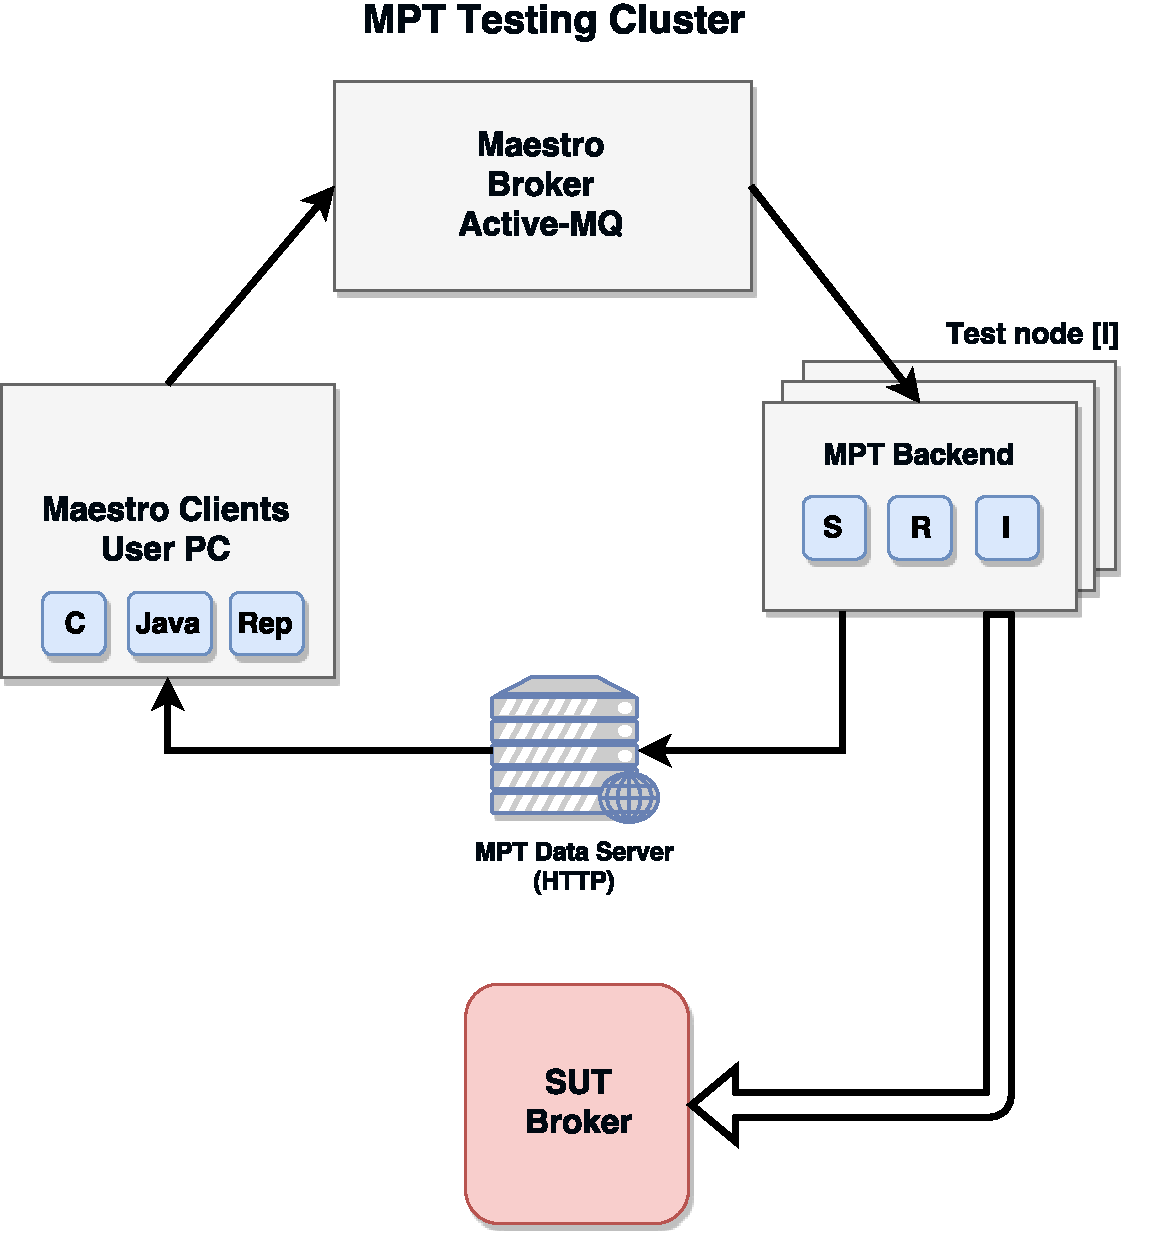
\includegraphics{figures/msg_perf_tool.pdf}}
           		\end{tabular} \\
			\end{tabular}					
		\end{frame}
		%/////////////////////////////////////////////////
		\section{Messaging Performance Tool}
		\begin{frame}{Messaging Performance Tool}
       		\begin{tabular}{cl}  
           		\begin{tabular}{l}
             		\parbox{0.37\linewidth}{%  change the parbox width as appropiate
						\begin{itemize}
							\item Maestro Clients update (New Commands)
							\item New component: Agent
							\item Ability to change topology (Shut down router, etc.)
						\end{itemize}
   					}
         		\end{tabular} 
         		& \begin{tabular}{l}
           			\scalebox{0.32}{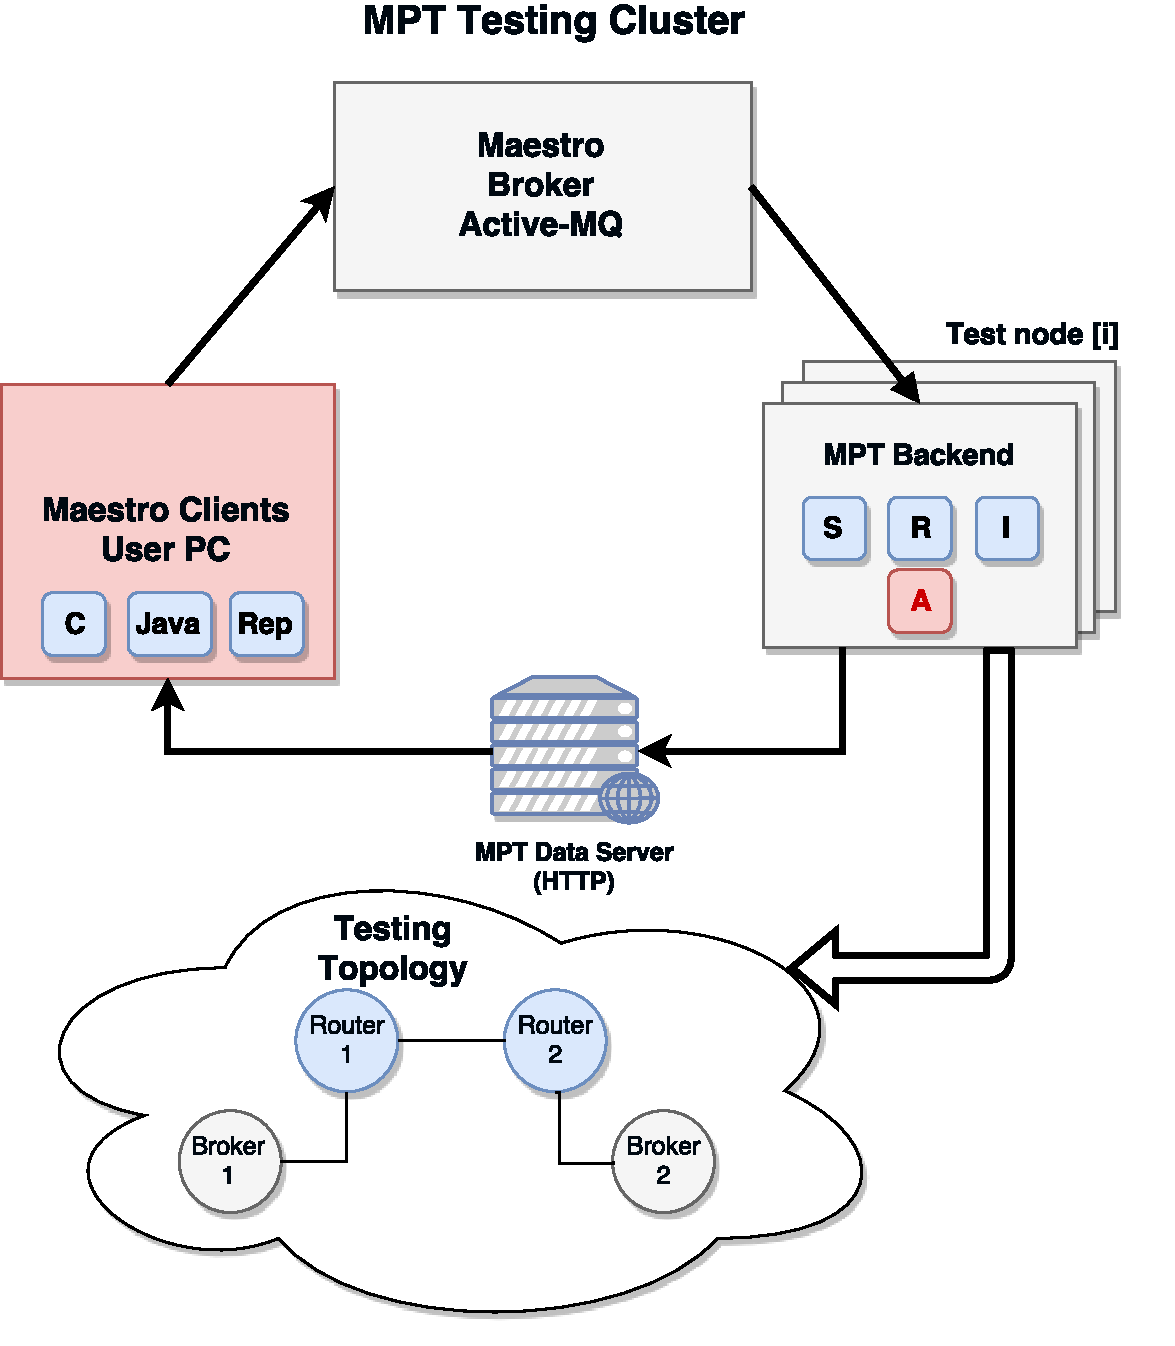
\includegraphics{figures/msg_perf_tool_for_router.pdf}}
           		\end{tabular} \\
			\end{tabular}	
		\end{frame}		
		%/////////////////////////////////////////////////
		\section{Topology Generator}
		\begin{frame}{Topology Generator}
       		\begin{tabular}{cl}  
           		\begin{tabular}{l}
             		\parbox{0.4\linewidth}{%  change the parbox width as appropiate
						\begin{itemize}
							\item Metadata $\rightarrow$ Configuration files
							\item Metadata are Inventory or Graph File
							\item Config based on Qpid-Dispatch version 
							\item Auto deployment by Ansible
						\end{itemize}
   					}
         		\end{tabular} 
         		& \begin{tabular}{l}
           			\scalebox{0.3}{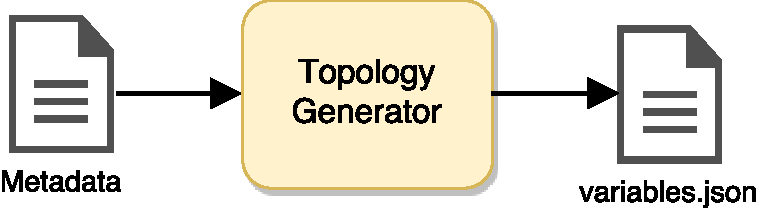
\includegraphics{figures/generator.pdf}} \\ \\ \\
           			\scalebox{0.3}{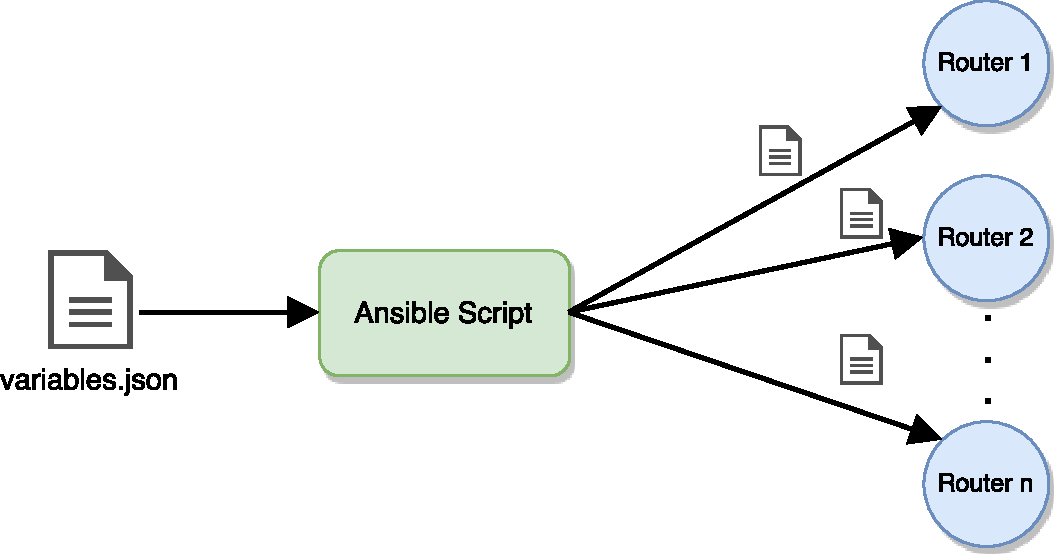
\includegraphics{figures/deployment.pdf}}
           		\end{tabular} \\
			\end{tabular}						
		\end{frame}
		%/////////////////////////////////////////////////
		\section{Summary}
		\begin{frame}{Summary}
				\begin{itemize}
						\item Upgrade of Messaging Performance Tool
						\begin{itemize}
							\item Add new commands to Maestro Clients
							\item Implement Qpid-Dispatch Agent
						\end{itemize}
						\item Improvements of Topology Generator
						\item Qpid-Dispatch performance measurements
						\item Experiments with Qpid-Dispatch recovery
				\end{itemize}
		\end{frame}
		%/////////////////////////////////////////////////
\end{document}
